%\subsection*{Statement of authorship}
\renewcommand{\arraystretch}{1.5}
\begin{tabular}{m{0.25\textwidth} m{0.67\textwidth}}
    \hline \hline Paper title & Analytic Magnetic Fields and Semi-Analytic Forces and Torques Due to General Polyhedral Permanent Magnets \\ \hline
    Publication status & Published \\ \hline
    Publication details & J. L. G. O’Connell, W. S. P. Robertson, and B. S. Cazzolato, ``Analytic Magnetic Fields and Semi-Analytic Forces and Torques Due to General Polyhedral Permanent Magnets,'' in IEEE Transactions on Magnetics, vol. 56, no. 1, Jan. 2020, doi: 10.1109/TMAG.2019.2942538. \\ \hline \hline
\end{tabular}

\vfill

\subsection*{Principal author}
\begin{tabular}{p{0.25\textwidth} m{0.67\textwidth}}
    \hline \hline Name & James O'Connell \\ \hline
    Contribution & \begin{itemize}
        \setlength\itemsep{-2mm}
        \item[-] Idea conceptualisation
        \item[-] Review of relevant literature
        \item[-] Performed all mathematical analysis, including derivation of solved field equations and estimated force and torque expressions
        \item[-] Implemented all algorithms and equations in MATLAB code, including considerable code testing and improvement to increase computation speed
        \item[-] Validation of methodology, including creation of finite element simulations and data analysis
        \item[-] Performed optimisation of magnet geometry to optimise field strength at a particular point in space
        \item[-] Wrote manuscript draft and created all figures
        \item[-] Finalisation of article
        \item[-] Preparation and submission for publication, including author correspondence
    \end{itemize} \\ \hline
    Percentage & 90\% \\ \hline
    Certification & This paper reports on original research conducted by the author during the period of Higher Degree by Research candidature and is not subject to any obligations or contractual agreements with a third party that would constrain its inclusion in this thesis. The author listed above is the primary author of this paper. \\ \hline
    Signature & \begin{tabular}{m{45mm} m{10mm} m{20mm}}
    \vspace{0.5mm}\includegraphics[width=0.3\textwidth]{jamesSignature.PNG} & Date: & 8 Dec 2021
    \end{tabular} \\ \hline
\end{tabular}

\vfill
    
\subsection*{Co-author contributions}
By signing this statement of authorship, each author certifies that:
\begin{enumerate}
    \item the candidate's stated contribution to the publication is accurate (as detailed above);
    \item permission is granted for the candidate to include the publication in the thesis; and
    \item the sum of all co-author contributions is equal to 100\% less the candidate's stated contribution.
\end{enumerate}
\begin{tabular}{m{0.25\textwidth} m{0.67\textwidth}}
    \hline \hline Name & Will Robertson \\ \hline
    Contribution & 5\% \\ \hline
    Signature & \vspace{2mm}\includegraphics[height=10mm]{willSig} \\  \hline
    Date & 16 Dec 2021 \\
    \hline \hline Name & Ben Cazzolato \\ \hline
    Contribution & 5\% \\ \hline
    Signature & \vspace{2mm} \includegraphics[height=10mm]{benSig} \\ \hline
    Date & 16 Dec 2021 \\
    \hline \hline \vfill
\end{tabular}
\renewcommand{\arraystretch}{1}
\newpage
%
\section*{\LARGE Analytic magnetic fields and semi-analytic forces and torques due to general polyhedral permanent magnets}
James L.G. O'Connell, William S.P. Robertson, and Benjamin S. Cazzolato
\section*{Abstract}\addcontentsline{toc}{section}{\protect\numberline{}Abstract}\label{sec:p1abstract}
This paper outlines an algorithm which analytically calculates the magnetic field produced by a general polyhedral permanent magnet with any number of faces and arbitrary face orientations, then uses the algorithm to \mbox{semi-analytically} calculate the force and torque on a second general polyhedral magnet. The algorithm is validated against both literature and finite element simulations using cuboids and dodecahedra. It is then used to model a basic two-magnet repulsive system, where it is shown that frustum magnets can produce a larger force per unit volume than cuboidal magnets. The shape of the frustums is optimised to maximise the force between them at a given separation distance, showing a considerable increase in force when compared to cuboidal magnets with the same volume. This paper shows that there is scope to improve performance of magnetic systems by using novel magnet shapes, and presents an algorithm which can be used for this optimisation process.
\section{Introduction}\label{sec:p1introduction}
Permanent magnets have many applications in magnetic resonance imaging, gearing, actuators, and motors \cite{Furlani2001}. Furthermore, they can be an essential component in wave energy harvesting \cite{Mann2010}, vibration isolation \cite{Robertson2009}, and many other applications. Due to their extensive use in a number of industries, it is important to understand the interactions between them, improving the design and optimisation process of electromagnetic systems.

Throughout recent decades, researchers have attempted to understand interactions between permanent magnets. \textcite{Akoun1984} started this trend by calculating the force between two parallel cuboidal permanent magnets with parallel magnetisation by finding the interaction energy between the magnets. \textcite{Janssen2010} used the same energy-based approach, but instead calculated the torque on one of the magnets. \textcite{Allag2009} extended the force and torque expressions to non-parallel magnetisations. \textcite{EngelHerbert2005} and \textcite{Ravaud2009} have calculated the magnetic field of cuboidal magnets rather than forces and torques. However, these studies are limited to cuboidal magnets and cannot be used for any other shapes.

A number of studies have examined ring and cylindrical magnets rather than cuboids. \textcite{Furlani1995} was able to semi-analytically calculate the field due to radially magnetised ring magnet sectors. Several papers by Ravaud et al.\ \cite{Ravaud2008,Ravaud2008a,Ravaud2009a} have found expressions for radially and axially magnetised ring magnets and sectors. Again, however, these studies are limited to ring magnets and cannot be used for other geometries.

To mitigate this geometrical limitation, some researchers have explored polyhedral permanent magnets, generalising the solution to any three dimensional shape with flat facets. Some authors such as \textcite{Soltner2010} and \textcite{Meessen2008} have approximated the magnetic field of a polyhedral magnet using assumptions such as the dipole model or discretisation of shapes into cuboids, but these are not always accurate. Other authors, however, have been more successful in solving for the exact magnetic field. \textcite{Janssen2010a} and \textcite{Rubeck2013} were able to find analytic expressions for the magnetic field of a polyhedral magnet by decomposing it into a collection of simple two-dimensional planar surfaces. \textcite{Meessen2008} and \textcite{Lee2004} studied trapezoidal magnets in a Halbach array using discretised magnets and magnets of infinite thickness respectively and found improvement in the maximum magnetic field strength over more traditional cuboidal Halbach arrays. However, there has been little work on the forces and torques due to polyhedral permanent magnets.

Several studies by \textcite{Beleggia2003,Beleggia2005}, \textcite{Beleggia2004}, and \textcite{DeGraef2009} examine magnetic nanoparticles with arbitrary shape. They found expressions for the demagnetisation tensor field, interaction energy, force, and torque using a Fourier space approach. However, for most shapes, these must be calculated numerically, limiting the accuracy and speed of the solution.

This paper outlines a semi-analytic method for calculating the magnetic fields, forces, and torques for polyhedral permanent magnets. First, an algorithm to analytically calculate the magnetic field is presented. This method is similar to the magnetic field calculation method given by \textcite{Rubeck2013} but requires evaluation of fewer terms by using general scalene triangles rather than right-angled triangles. Then, numeric integration is performed to find the force and torque on a second polyhedral magnet due to the field from the first. This work is validated using past literature and finite element simulations on the magnetic configuration presented by \textcite{Akoun1984}. To further validate the algorithm, finite element simulations are performed on two perpendicularly magnetised dodecahedral magnets, which are compared to the semi-analytic solutions from this method. Once validated, a configuration involving two pyramidal frustum magnets is presented, where it is shown that the frustums can produce a larger repulsive force per unit volume than cuboidal magnets. Finally, this algorithm is used to optimise the geometry of the frustums to maximise the force between them.
\section{Methodology}\label{sec:p1methodology}
This work uses the charge method outlined by \textcite{Furlani2001}, where a fictitious magnetic charge is distributed over the surface of each magnet, and assumes a relative permeability \(\mu_r\) of unity with constant uniform magnetisation \(\mathbf{M}\). Recent studies have detailed methods for including the effect of non-unity permeability in calculations of the magnetic field from permanent magnets \cite{Dam2016}. While out of the scope for the current work, such methods can also be applied to the results presented here.

In this method, polyhedral permanent magnets are decomposed into the polygonal facets that make up the surface of the polyhedron. Each polygonal facet has a fictitious magnetic charge distribution, which creates a magnetic field and thus induces forces and torques on other magnets.

In this work, two magnets are defined, magnet A and magnet B. The force and torque on magnet B is calculated due to the field produced by magnet A. An algorithm to analytically calculate the field due to magnet A is presented. Then, a mesh is applied to the surface of magnet B and the field due to magnet A is calculated at each mesh element. Finally, numeric integration is performed to find the force and torque on magnet B. These steps are outlined in more detail below.
\begin{figure*}
	\centering
	\begin{subfigure}{0.4\textwidth}
		\centering
		\tdplotsetmaincoords{70}{110}
		\tdplotsetrotatedcoords{0}{0}{0}
		\begin{tikzpicture}[scale = 0.45,tdplot_rotated_coords]
		
		\coordinate (p1b) at (0,1,5);
		\coordinate (p2b) at (0,3,5);
		\coordinate (p3b) at (0,6,3);
		\coordinate (p4b) at (0,6,-2);
		\coordinate (p5b) at (0,1,-2);
		\coordinate (p1f) at (5,1,5);
		\coordinate (p2f) at (5,3,5);
		\coordinate (p3f) at (5,6,3);
		\coordinate (p4f) at (5,6,-2);
		\coordinate (p5f) at (5,1,-2);
		
		\draw (p1b) -- (p2b) -- (p3b) -- (p4b);% -- (p5b) -- cycle;
		\draw[fill=black!10] (p1f) -- (p2f) -- (p3f) -- (p4f) -- (p5f) -- cycle;
		\draw (p1f) -- (p1b);
		\draw (p2f) -- (p2b);
		\draw (p3f) -- (p3b);
		\draw (p4f) -- (p4b);
		
		\draw[->,thick] (5,3.5,0.5) -- (5,3.5,2.5);
		\node (M1) at (5,4,1.5) {\textbf{M}};
		\end{tikzpicture}
		\caption{}
		\label{fig:p13dpolyhedron}
	\end{subfigure}
	
	\vspace{20pt}
	
	\begin{subfigure}{0.4\textwidth}
		\centering
		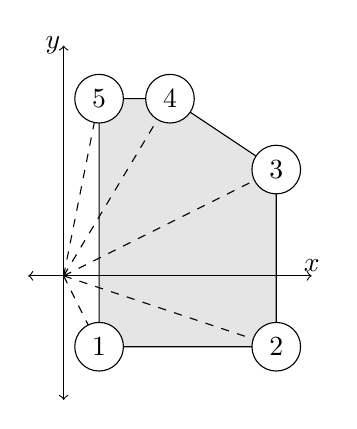
\begin{tikzpicture}[scale=0.45]
		\coordinate (origin) at (0,0);
		\coordinate (p5) at (1,5);
		\coordinate (p4) at (3,5);
		\coordinate (p3) at (6,3);
		\coordinate (p2) at (6,-2);
		\coordinate (p1) at (1,-2);
		
		\filldraw[fill = black!10] (p1) -- (p2) -- (p3) -- (p4) -- (p5) -- cycle;
		
		\draw[dashed] (origin) node {} -- (p1) node[circle,fill=white,draw,solid] {1};
		\draw[dashed] (origin) node {} -- (p2) node[circle,fill=white,draw,solid] {2};
		\draw[dashed] (origin) node {} -- (p3) node[circle,fill=white,draw,solid] {3};
		\draw[dashed] (origin) node {} -- (p4) node[circle,fill=white,draw,solid] {4};
		\draw[dashed] (origin) node {} -- (p5) node[circle,fill=white,draw,solid] {5};
		
		\node (x) at (7,0.3){\(x\)};
		\node (y) at (-0.3,6.5){\(y\)};
		
		\draw [<->] (-1,0) -- (7,0);
		\draw [<->] (0,-3.5) -- (0,6.5);
		\end{tikzpicture}
		\caption{}
		\label{fig:p1polygondecomposition}
	\end{subfigure}
	~
	\begin{subfigure}{0.4\textwidth}
		\centering
		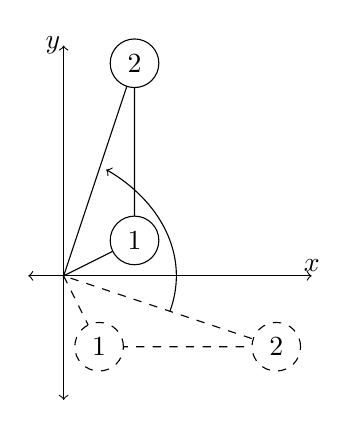
\begin{tikzpicture}[scale=0.45]
		\coordinate (origin) at (0,0);
		\coordinate (p2) at (2,1);
		\coordinate (p1) at (2,6);
		
		\draw[solid] (p1) -- (origin) -- (p2) -- cycle;
		\path (p1) node[circle,fill=white,draw,solid] {2} -- (p2) node[circle,fill=white,draw,solid] {1};
		
		\draw[dashed] (0,0) -- (1,-2) -- (6,-2) -- cycle;
		\path (6,-2) node[circle,fill=white,draw,dashed] {2} -- (1,-2) node[circle,fill=white,draw,dashed] {1};
		
		\node (x) at (7,0.3){\(x\)};
		\node (y) at (-0.3,6.5){\(y\)};
		
		\draw [<->] (-1,0) -- (7,0);
		\draw [<->] (0,-3.5) -- (0,6.5);
		
		\draw[<-] (1.2,3) to [out=-30,in=70] (3,-1.0);
		\end{tikzpicture}
		\caption{}
		\label{fig:p1makingtriangles}
	\end{subfigure}
	\caption{A simple polyhedral permanent magnet, created by chamfering one edge of a cuboid (a). The magnet is magnetised vertically upward, as indicated by the arrow. Each facet is rotated such that it is parallel to the \(XY\)-plane and a line is drawn from the \(z\)-axis to each vertex (b), creating \(n\) triangles from the \(n\)-sided facet. Each triangle is rotated such that the edge joining the two vertices is parallel to the \(y\)-axis (c). The field of each rotated triangle is calculated then rotated back to the initial state. Each of these fields is added to give the total field of the facet. This process is then repeated for all other facets of the polyhedron to give the total field of the polyhedron.}
	\label{fig:p1decomposethepolygon}
\end{figure*}

\subsection{Calculation of the field due to magnet A}
The field due to magnet A is found using a similar method to \textcite{Rubeck2013}, but the equations are more efficient. Unlike the field equations presented by \textcite{Janssen2010}, all expressions and sub-expressions here are purely real. The magnetic field is found by first taking a polyhedral permanent magnet, such as that shown in Figure \ref{fig:p13dpolyhedron}\footnote{The magnet shown in Figure \ref{fig:p1decomposethepolygon} is a 5 unit (width) by 7 unit (height) by 5 unit (depth) cuboid, with a chamfer cutting the top face to a width of 2 units and one of the vertical faces to a height of 5 units.}, and decomposing it into its polygonal facets. Each facet is rotated about the \(x\)- and \(y\)-axes, making it parallel to the \(XY\)-plane, using the rotation matrix \(R_{xy}\), given by
\begin{equation}
R_{xy} = \begin{bmatrix}
\frac{n_z}{\sqrt{n_x^2+n_z^2}} & 0 & -\frac{n_x}{\sqrt{n_x^2+n_z^2}} \\
-\frac{n_xn_y}{\sqrt{n_x^2+n_z^2}} & \sqrt{n_x^2+n_z^2} & \frac{n_yn_z}{\sqrt{n_x^2+n_z^2}} \\
n_x & n_y & n_z
\end{bmatrix} \text{,}
\end{equation}
\noindent where \(\hat{\mathbf{n}} = \left[ n_x, n_y, n_z \right]\) is the outward-facing unit normal vector of each facet. Once parallel to the \(XY\)-plane, a line is drawn from the \(z\)-axis to each polygon vertex, as shown in Figure \ref{fig:p1polygondecomposition}, forming \(n\) triangles, where \(n\) is the number of sides of the polygon. It is important that the last triangle is defined from vertex \(n\) to vertex 1. This is because this algorithm calculates the field due to each triangle, which may include area not covered by the polygon. For example, the triangle between the \(z\)-axis, vertex 1, and vertex 5 of the polygon shown in Figure \ref{fig:p1polygondecomposition} is not part of the polygon, but the field of it is calculated from the first four triangles. The fifth triangle is defined from vertex 5 to vertex 1, effectively creating a triangle which subtracts the field due to this area outside the polygon.

After \(n\) triangles have been defined, each one is rotated so that the side joining the two vertices is parallel to the \(y\)-axis, shown in Figure \ref{fig:p1makingtriangles}. This is done using the rotation matrix
\begin{equation}
R_z = \begin{bmatrix}
-\frac{y_2-y_1}{\sqrt{\left( y_2-y_1 \right)^2 + \left( x_2-x_1 \right)^2}} & \frac{x_2-x_1}{\sqrt{\left( y_2-y_1 \right)^2 + \left( x_2-x_1 \right)^2}} & 0 \\
-\frac{x_2-x_1}{\sqrt{\left( y_2-y_1 \right)^2 + \left( x_2-x_1 \right)^2}} & -\frac{y_2-y_1}{\sqrt{\left( y_2-y_1 \right)^2 + \left( x_2-x_1 \right)^2}} & 0 \\
0 & 0 & 1
\end{bmatrix} \text{,}\\
\end{equation}
\noindent where \(x_1\), \(x_2\), \(y_1\), and \(y_2\) are the \(x\) and \(y\) coordinates of the two vertices not intersecting the \(z\)-axis before the triangle is rotated.

After rotation, the charge model outlined by \textcite{Furlani2001} can be used to solve for the magnetic field due to each triangle using the following expression.
\begin{eqnarray}\label{eqn:p1chargeB}
\mathbf{B} = -\frac{\mu_0}{4\pi} \int_{V} \left( \nabla \cdot \mathbf{M} \right) \frac{\mathbf{x} - \mathbf{x}'}{\left| \mathbf{x} - \mathbf{x}' \right|^3} \ dv' + \frac{\mu_0}{4\pi} \oint_{S} \left( \mathbf{M} \cdot \hat{\mathbf{n}} \right) \frac{\mathbf{x} - \mathbf{x}'}{\left| \mathbf{x} - \mathbf{x}' \right|^3} \ ds' \text{,}
\end{eqnarray}
\noindent where \(\mathbf{B}\) is the magnetic field, \(\mu_0\) is the magnetic permeability of free space, \(\mathbf{M}\) is the magnetisation vector, \(\mathbf{x}\) is the point of interest, \(\mathbf{x}'\) is a point on or inside the magnet, \(d{\mathrm{v}}'\) is a volume element of the magnet, and \(d{\mathrm{s}}'\) is a surface element of the magnet.

Assuming constant uniform magnetisation \(\mathbf{M}\), the first integral in Equation (\ref{eqn:p1chargeB}) disappears as \(\nabla \cdot \mathbf{M}=0\). The magnetic field due to each triangle can then be found by solving the second integral, giving
\begin{align}\label{eqn:p1trieqns}
    B_{x\Delta} &= \frac{\mu_0 \mathbf{M} \cdot \mathbf{\hat{n}}}{4\pi} \left( \frac{1}{2}\log\frac{\left( l_{az2}+y_2\right)\left(l_{az1}-y_1\right)}{\left(l_{az2}-y_2\right)\left(l_{az1}+y_1\right)} + \right. \nonumber \\
	& \quad \quad \quad \quad \quad \quad \quad \left. \frac{y_1}{2l_{a1}} \log \frac{l_{az1}+l_{a1}}{l_{az1}-l_{a1}} - \frac{y_2}{2l_{a2}} \log \frac{l_{az2}+l_{a2}}{l_{az2}-l_{a2}} \right) \nonumber \\
    & \quad \nonumber \\
	B_{y\Delta} &= \frac{\mu_0 \mathbf{M} \cdot \mathbf{\hat{n}}}{4\pi} \left( \frac{a}{2l_{a2}} \log \frac{l_{az2}+l_{a2}}{l_{az2}-l_{a2}} - \frac{a}{2l_{a1}} \log \frac{l_{az1}+l_{a1}}{l_{az1}-l_{a1}} \right) \\
    & \quad \nonumber \\
	B_{z\Delta} &= -\frac{\mu_0 \mathbf{M} \cdot \mathbf{\hat{n}}}{4\pi} \left( \text{sgn} \left( z' \right) \arctan \frac{ay_2-ay_1}{y_1y_2+a^2} + \right. \nonumber \\
	& \quad \quad \quad \quad \quad \quad \quad \left. \arctan \frac{az'y_1l_{az2}-az'y_2l_{az1}}{z'^2y_1y_2+a^2l_{az1}l_{az2}} \right)  \text{,} \nonumber
\end{align}
%\begin{subequations}
%	\begin{eqnarray}
%	B_{x\Delta} &=& \frac{\mu_0 \mathbf{M} \cdot \mathbf{\hat{n}}}{4\pi} \left( \frac{1}{2}\log\frac{\left( l_{az2}+y_2\right)\left(l_{az1}-y_1\right)}{\left(l_{az2}-y_2\right)\left(l_{az1}+y_1\right)} + \right. \nonumber \\
%	& & \left. \frac{y_1}{2l_{a1}} \log \frac{l_{az1}+l_{a1}}{l_{az1}-l_{a1}} - \frac{y_2}{2l_{a2}} \log \frac{l_{az2}+l_{a2}}{l_{az2}-l_{a2}} \right) \\
%	&&\nonumber\\
%	B_{y\Delta} &=& \frac{\mu_0 \mathbf{M} \cdot \mathbf{\hat{n}}}{4\pi} \left( \frac{a}{2l_{a2}} \log \frac{l_{az2}+l_{a2}}{l_{az2}-l_{a2}} - \right. \nonumber \\
%	& & \left. \frac{a}{2l_{a1}} \log \frac{l_{az1}+l_{a1}}{l_{az1}-l_{a1}} \right)  \\
%	&&\nonumber\\
%	B_{z\Delta} &=& -\frac{\mu_0 \mathbf{M} \cdot \mathbf{\hat{n}}}{4\pi} \left( \text{sgn} \left( z' \right) \arctan \frac{ay_2-ay_1}{y_1y_2+a^2} + \right. \nonumber \\
%	& & \left. \arctan \frac{az'y_1l_{az2}-az'y_2l_{az1}}{z'^2y_1y_2+a^2l_{az1}l_{az2}} \right)  \text{,}
%	\end{eqnarray}
%\end{subequations}
\noindent with
\begin{align*}
l_{a1} &= \sqrt{a^2+y_1^2} \nonumber \\
l_{a2} &= \sqrt{a^2+y_2^2} \nonumber \\
l_{az1} &= \sqrt{a^2+y_1^2+z'^2} \nonumber \\
l_{az2} &= \sqrt{a^2+y_2^2+z'^2} \nonumber \text{,}
\end{align*}
\noindent where \(\log()\) is the natural logarithm, \(\text{sgn}()\) is the sign function, \(\arctan()\) is the arctangent, and \(\left( 0,0,z' \right)\), \(\left( a,y_1,z' \right)\), and \(\left( a,y_2,z' \right)\) are the coordinates of the triangle vertices after rotation. This field can then be rotated back to the original position using the rotation matrix \(R_z^{-1}\). The field due to each triangle is summed, giving the field of the polygonal facet. Then, the field due to the polygonal facet is rotated back to the original position using the rotation matrix \(R_{xy}^{-1}\). The total field due to magnet A is then calculated by summing the field contribution of each polygonal facet. This field calculation gives the magnetic field at the origin, but the magnetic field at any point can be calculated using a coordinate translation such that the point of interest lies on the origin. The magnetic field calculation can be represented using Algorithm \ref{alg:p1alg1}.
\begin{algorithm}
	\caption{Calculate the magnetic field of a polyhedral permanent magnet}
	\begin{algorithmic}[1]
		\State Set \(\mathbf{B} = [0,0,0]^\textsf{T}\).
		\For {each \(n\)-sided facet of the polyhedron}
		\State \parbox[t]{\dimexpr\linewidth-\leftmargin-\labelsep-\labelwidth}{Define the vertices in an anticlockwise order when looking at the polyhedron from the outside.}\newline
		\State \parbox[t]{\dimexpr\linewidth-\leftmargin-\labelsep-\labelwidth}{Store these in a \(3\times n\) matrix \(P\) such that each column represents a vertex.}\newline
		\State \parbox[t]{\dimexpr\linewidth-\leftmargin-\labelsep-\labelwidth}{Copy the first column of \(P\) and add it as the \(\left(n+1\right)\)th column.}\newline
		\State \parbox[t]{\dimexpr\linewidth-\leftmargin-\labelsep-\labelwidth}{Evaluate the matrix \(R_{xy}\) and create a new matrix \(P_{xy}\) given by \(P_{xy} = R_{xy}P\).}\newline
		\For {\(j=1,\dots,n\)}
		\State \parbox[t]{\dimexpr\linewidth-\leftmargin-\labelsep-\labelwidth}{Using the \(j\)th and \(\left(j+1\right)\)th columns of \(P_{xy}\), calculate \(R_z\). Create \(P_z\) given by \(P_z = R_zP_{xy}\).}\newline
		\State \parbox[t]{\dimexpr\linewidth-\leftmargin-\labelsep-\labelwidth}{Evaluate \(\textbf{B}_\Delta\) using the points from \(P_z\) and Equation (\ref{eqn:p1trieqns}).}\newline
		\State \label{alg:p1enum2}Add the value of \(\left(R_{xy}^{-1}R_z^{-1}\textbf{B}_\Delta\right)\) to \(\mathbf{B}\).
		\EndFor
		\EndFor
		\State The field at the origin is now equal to \(\mathbf{B}\).
	\end{algorithmic}\label{alg:p1alg1}
\end{algorithm}

Algorithm \ref{alg:p1alg1} was implemented on the three-dimensional polyhedral magnet shown in Figure \ref{fig:p1decomposethepolygon}. Flux lines were drawn on the plane of symmetry to give a visual representation of the magnetic field, and are shown in Figure \ref{fig:p1fluxlines}.
\begin{figure}
	\centering
	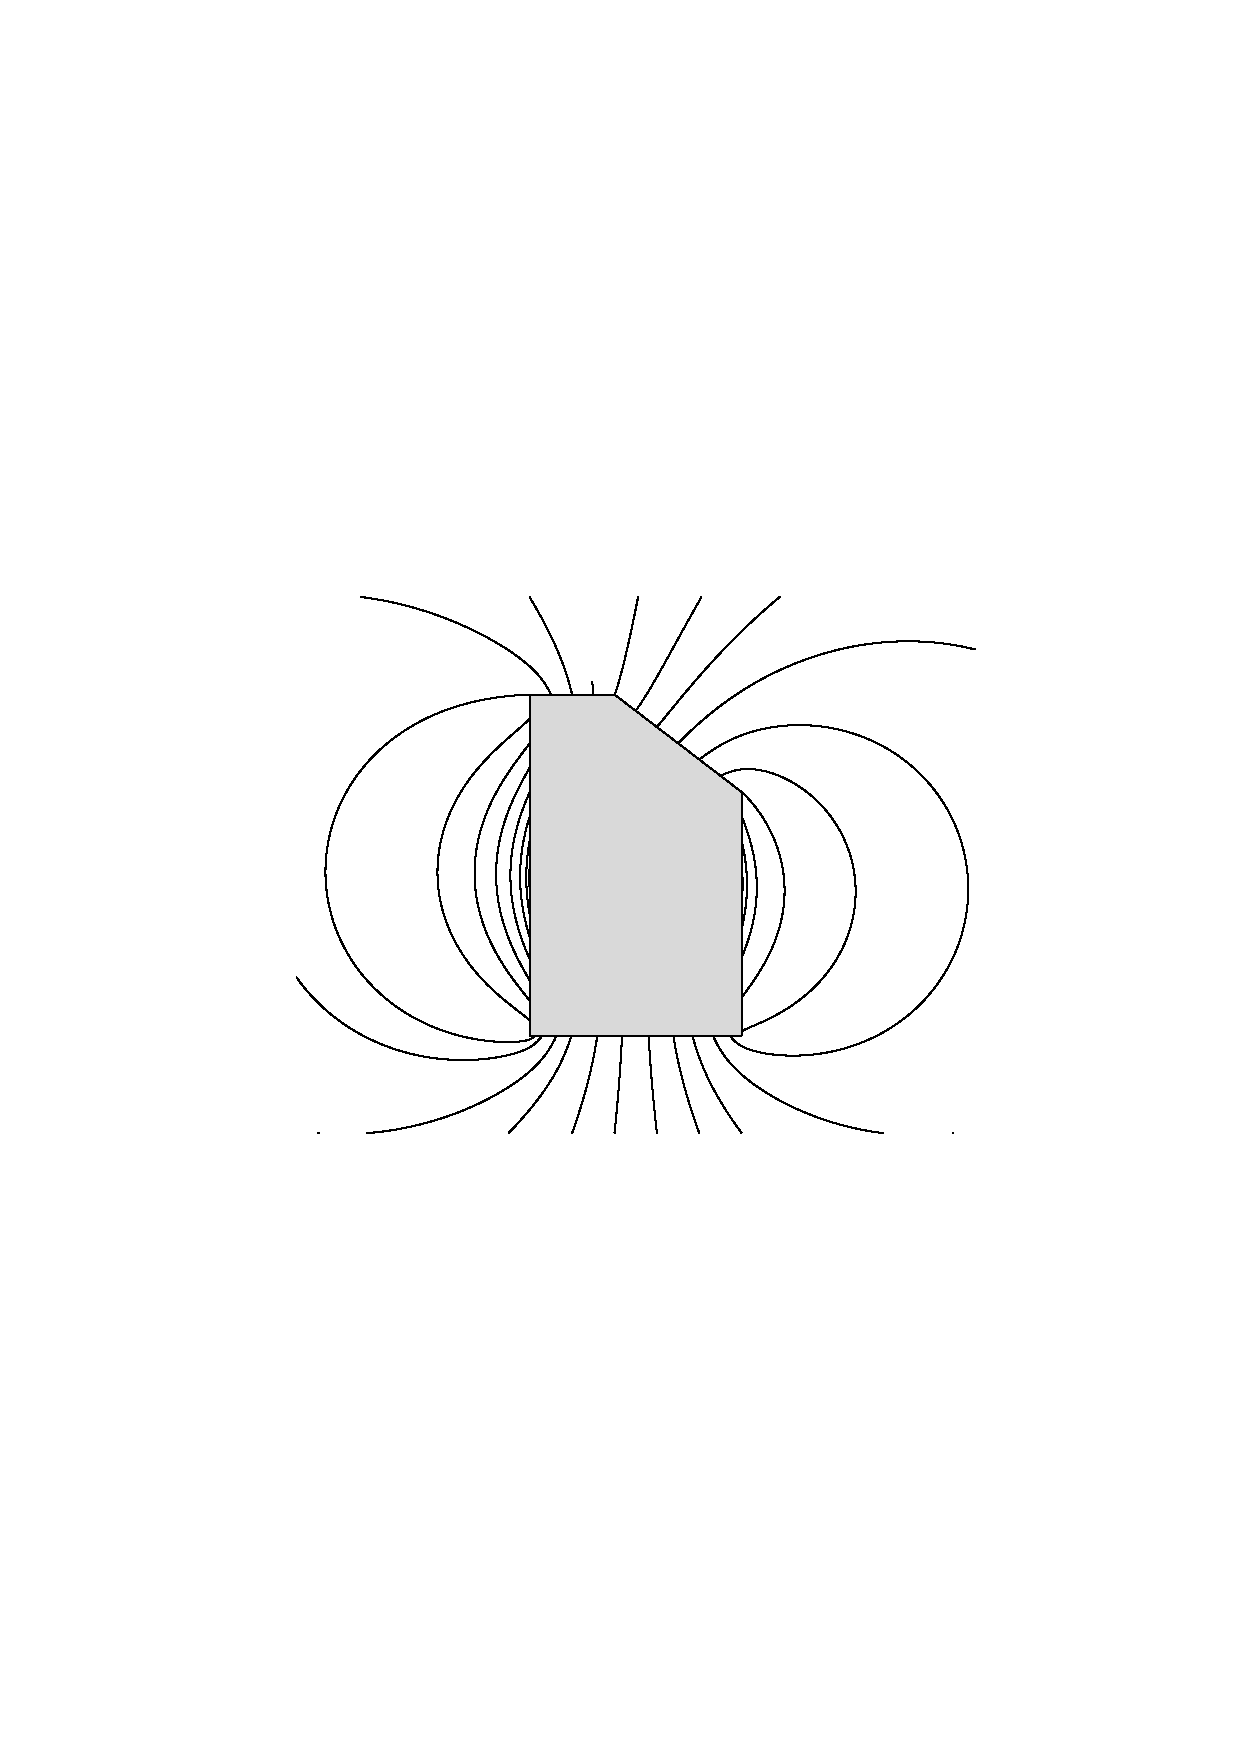
\includegraphics[trim = 3cm 10cm 3cm 10cm,width=0.8\linewidth]{p1/p1FIG2}
	\caption{The magnetic flux lines of the polyhedral magnet shown in Figure \ref{fig:p1decomposethepolygon}. The flux lines travel from the north pole (top) of the magnet to the south pole (bottom) of the magnet. The flux lines behave similarly to that of a cuboidal magnet in most regions due to the magnet being almost cuboidal. However, in the top right region, the flux lines differ from those of a cuboidal magnet due to the chamfer.}
	\label{fig:p1fluxlines}
\end{figure}

\subsection{Force and torque on magnet B}
The force and torque on magnet B is found using numeric integration of the magnetic field due to magnet A over the surface of magnet B, as described by \textcite{Furlani2001}. This is done by numerically solving the integrals
\begin{subequations}
    \begin{eqnarray}
	\mathbf{F}_\text{B} &=& \oint_{S_\text{B}} \left( \mathbf{M}_\text{B} \cdot \mathbf{\hat{n}}_\text{B} \right) \mathbf{B}_\text{A}\  ds_\text{B} \text{,} \\
	\mathbf{T}_\text{B} &=& \oint_{S_\text{B}} \left( \mathbf{M}_\text{B} \cdot \mathbf{\hat{n}}_\text{B} \right) \left( \mathbf{r}_\text{B} \times \mathbf{B}_\text{A} \right)\ ds_\text{B} \text{,}
	\end{eqnarray}
\end{subequations}
\noindent where \({S_\mathrm{B}}\) is the surface of magnet B, \({\mathbf{M}_\mathrm{B}}\) is the magnetisation vector of magnet B, \({\mathbf{\hat{n}}_\mathrm{B}}\) is the outward-facing normal vector of the surface of magnet B, \({\mathbf{B}_\mathrm{A}}\) is the field due to magnet A, and \({\mathbf{r}_\mathrm{B}}\) is the vector from the point of rotation of magnet B to the surface of magnet B.

To solve these expressions, a mesh is defined on the surface of magnet B. This mesh must be defined such that the field due to magnet A is relatively constant over each element. The field due to magnet A is evaluated at the centre of each mesh element using Algorithm \ref{alg:p1alg1}. The force and torque on magnet B can be found by numerically integrating the field at each element with area \(A_i\), as shown in Equation (\ref{eqn:p1numericforcetorque}), where \(\mathbf{b}_i\) is the field due to magnet A at the centre of each mesh element.
\begin{subequations}
	\label{eqn:p1numericforcetorque}
	\begin{eqnarray}
	\mathbf{F}_\text{B} &=& \sum_i \left( \mathbf{M}_\text{B} \cdot \mathbf{\hat{n}}_\text{B} \right) {\mathbf{b}_i A_i} \text{,} \\
	\mathbf{T}_\text{B} &=& \sum_i \left( \mathbf{M}_\text{B} \cdot \mathbf{\hat{n}}_\text{B} \right) \left( {\mathbf{r}_i \times \mathbf{b}_i} \right) A_i \text{.}
	\end{eqnarray}
\end{subequations}

This process can be represented programmatically using Algorithm \ref{alg:p1alg2}.
\begin{algorithm}
	\caption{Calculate the force and torque on a polyhedral permanent magnet}
	\begin{algorithmic}[1]
		\State Apply a mesh to the surface of magnet B.
		\For {each mesh element \(i\) on the surface of magnet B}
		\State \parbox[t]{\dimexpr\linewidth-\leftmargin-\labelsep-\labelwidth}{Translate the entire system so the centre of the element lies on the origin.}\newline
		\State \parbox[t]{\dimexpr\linewidth-\leftmargin-\labelsep-\labelwidth}{Calculate the magnetic field strength from magnet A using Algorithm \ref{alg:p1alg1}.}\newline
		\State \parbox[t]{\dimexpr\linewidth-\leftmargin-\labelsep-\labelwidth}{Calculate the cross product of the torque moment arm and the magnetic field strength \(\mathbf{r}\times\mathbf{b}\).}\newline
		\State Calculate the quantity \(\mathbf{M}\cdot\hat{\mathbf{n}}\) for the element.
		\State \parbox[t]{\dimexpr\linewidth-\leftmargin-\labelsep-\labelwidth+4mm}{Set \(\mathbf{f}_i=\left(\mathbf{M}\cdot\hat{\mathbf{n}}\right)\mathbf{b}A_i\) and \(\mathbf{\tau}_i=\left(\mathbf{M}\cdot\hat{\mathbf{n}}\right)\left(\mathbf{r}\times\mathbf{b}\right)A_i\) where \(A_i\) is the area of the element.}\newline
		\EndFor
		\State {Set \(\mathbf{F} = \sum_i\mathbf{f}_i\) and \(\mathbf{T} = \sum_i\mathbf{\tau}_i\).}
		\State The force and torque on magnet B are given by \(\mathbf{F}\) and \(\mathbf{T}\) respectively.
	\end{algorithmic}\label{alg:p1alg2}
\end{algorithm}

Thus the exact magnetic field due to a polyhedral permanent magnet has been analytically calculated, and the force and torque on a second polyhedral magnet has been numerically calculated using the analytic field solution.
\section{Validation}\label{sec:p1validation}
The field, force, and torque solutions outlined in Section \ref{sec:p1methodology} have been verified using both previous literature and finite element simulations. Firstly, the configuration used by \textcite{Akoun1984}\footnote{\textcite{Akoun1984} used two cuboidal magnets, each of dimensions 20mm by 12mm by 6mm with a vertical gap of 2mm between them.} was considered (Figure \ref{fig:p1akounyonnet}). Here, the force on magnet B is measured as it moves a distance \(d\) in the \(x\)-direction while magnet A remains fixed. Both magnets have parallel magnetisation vectors in the \(z\)-direction with a value of 0.38 Tesla. The resulting force and torque depends not only on magnetisation, but also on the geometry of the magnets.
\begin{figure*}
	\centering
	\begin{subfigure}{0.4\textwidth}
		\centering
		\tdplotsetmaincoords{70}{130}
		\begin{tikzpicture}[scale=0.2,tdplot_main_coords]
		\coordinate(b1) at (10,-6,3);
		\coordinate(b2) at (10,6,3);
		\coordinate(b3) at (-10,6,3);
		\coordinate(b4) at (-10,-6,3);
		\coordinate(b5) at (10,-6,-3);
		\coordinate(b6) at (10,6,-3);
		\coordinate(b7) at (-10,6,-3);
		
		\draw (b1) -- (b2) -- (b3) -- (b4) -- cycle;
		\draw (b5) -- (b6) -- (b7);
		\draw (b1) -- (b5);
		\draw (b2) -- (b6);
		\draw (b3) -- (b7);
		
		\coordinate(t1) at (2,-14,11);
		\coordinate(t2) at (2,6,11);
		\coordinate(t3) at (-10,6,11);
		\coordinate(t4) at (-10,-14,11);
		\coordinate(t5) at (2,-14,5);
		\coordinate(t6) at (2,6,5);
		\coordinate(t7) at (-10,6,5);
		
		\draw[fill=white] (t1) -- (t2) -- (t6) -- (t5);
		\draw[fill=white] (t2) -- (t3) -- (t7) -- (t6);
		\draw (t5) -- (t1) -- (t4) -- (t3);
		
		\coordinate(midpt) at (2,-4,8);
		\coordinate(end) at (12,-4,8);
		
		\draw[->,dashed] (midpt) -- (end);
		
		\node(d) at (14.5,-3,8.5) {\textit{d}};
		\node(A) at (0,6,0) {\text{A}};
		\node(B) at (-4,6,8) {\text{B}};
		\end{tikzpicture}
		\caption{}
	\end{subfigure}
	~ \hspace{1cm}
	\begin{subfigure}{0.4\textwidth}
		\centering
		\tdplotsetmaincoords{90}{180}
		\begin{tikzpicture}[scale=0.2,tdplot_main_coords]
		\coordinate(b1) at (10,-6,3);
		\coordinate(b2) at (10,6,3);
		\coordinate(b3) at (-10,6,3);
		\coordinate(b4) at (-10,-6,3);
		\coordinate(b5) at (10,-6,-3);
		\coordinate(b6) at (10,6,-3);
		\coordinate(b7) at (-10,6,-3);
		
		\draw (b1) -- (b2) -- (b3) -- (b4) -- cycle;
		\draw (b5) -- (b6) -- (b7);
		\draw (b1) -- (b5);
		\draw (b2) -- (b6);
		\draw (b3) -- (b7);
		
		\coordinate(t1) at (2,-14,11);
		\coordinate(t2) at (2,6,11);
		\coordinate(t3) at (-10,6,11);
		\coordinate(t4) at (-10,-14,11);
		\coordinate(t5) at (2,-14,5);
		\coordinate(t6) at (2,6,5);
		\coordinate(t7) at (-10,6,5);
		
		\draw[fill=white] (t1) -- (t2) -- (t6) -- (t5);
		\draw[fill=white] (t2) -- (t3) -- (t7) -- (t6);
		\draw (t5) -- (t1) -- (t4) -- (t3);
		
		\coordinate(midpt) at (2,-4,8);
		\coordinate(end) at (6,-4,8);
		
		\draw[->,dashed] (midpt) -- (end);
		\node(d) at (7,-3,8) {\textit{d}};
		
		\draw[->,thick] (-4,0,6.5) -- (-4,0,9.5);
		\node (M1) at (-2.5,0,8) {\textbf{M}};
		\draw[->,thick] (0,0,-1.5) -- (0,0,1.5);
		\node (M2) at (1.5,0,0) {\textbf{M}};
		
		\node (A) at (-8,6,0) {\text{A}};
		\node(B) at (-8,6,8) {\text{B}};
		
		\draw [->] (-15,-4,-3) -- (-12,-4,-3);
		\draw [->] (-15,-4,-3) -- (-15,-4,0);
		\node (x) at (-11,-4,-3) {\(x\)};
		\node (z) at (-15,-4,1) {\(z\)};
		\end{tikzpicture}
		\caption{}
	\end{subfigure}
	\caption{The geometry used in Akoun and Yonnet's work in 1984 \cite{Akoun1984} with both magnets having parallel magnetisation in the \(z\)-direction. Magnet B moves a distance \(d\) along the top of magnet A.}
	\label{fig:p1akounyonnet}
\end{figure*}

Algorithms \ref{alg:p1alg1} and \ref{alg:p1alg2} were implemented in Matlab R2017b (MathWorks, Inc., Natick, MA, USA), with a basic meshing process using triangular elements. The mesh was created by repeatedly bisecting each triangle edge and joining the three bisection points, converting the triangle into four smaller triangles, until all triangles in the mesh had area less than a threshold value. Algorithms \ref{alg:p1alg1} and \ref{alg:p1alg2} were applied to Akoun and Yonnet's geometry \cite{Akoun1984} to calculate force and torque values for varying displacement. The finite element package Maxwell3D in ANSYS Electronics Desktop 2018.0 (ANSYS, Inc., Berkeley, CA, USA) was used with adaptive meshing to obtain finite element solutions for the force and torque in this configuration. Additionally, the force solutions presented by \textcite{Akoun1984} and torque solutions presented by \textcite{Janssen2010a} were calculated using Matlab code from Robertson \cite{Robertson2013,Robertson}, with the torque being evaluated about the centre of magnet B. These results were compared to those obtained with Algorithms \ref{alg:p1alg1} and \ref{alg:p1alg2} as well as finite element simulations.
\begin{figure*}
	\centering
	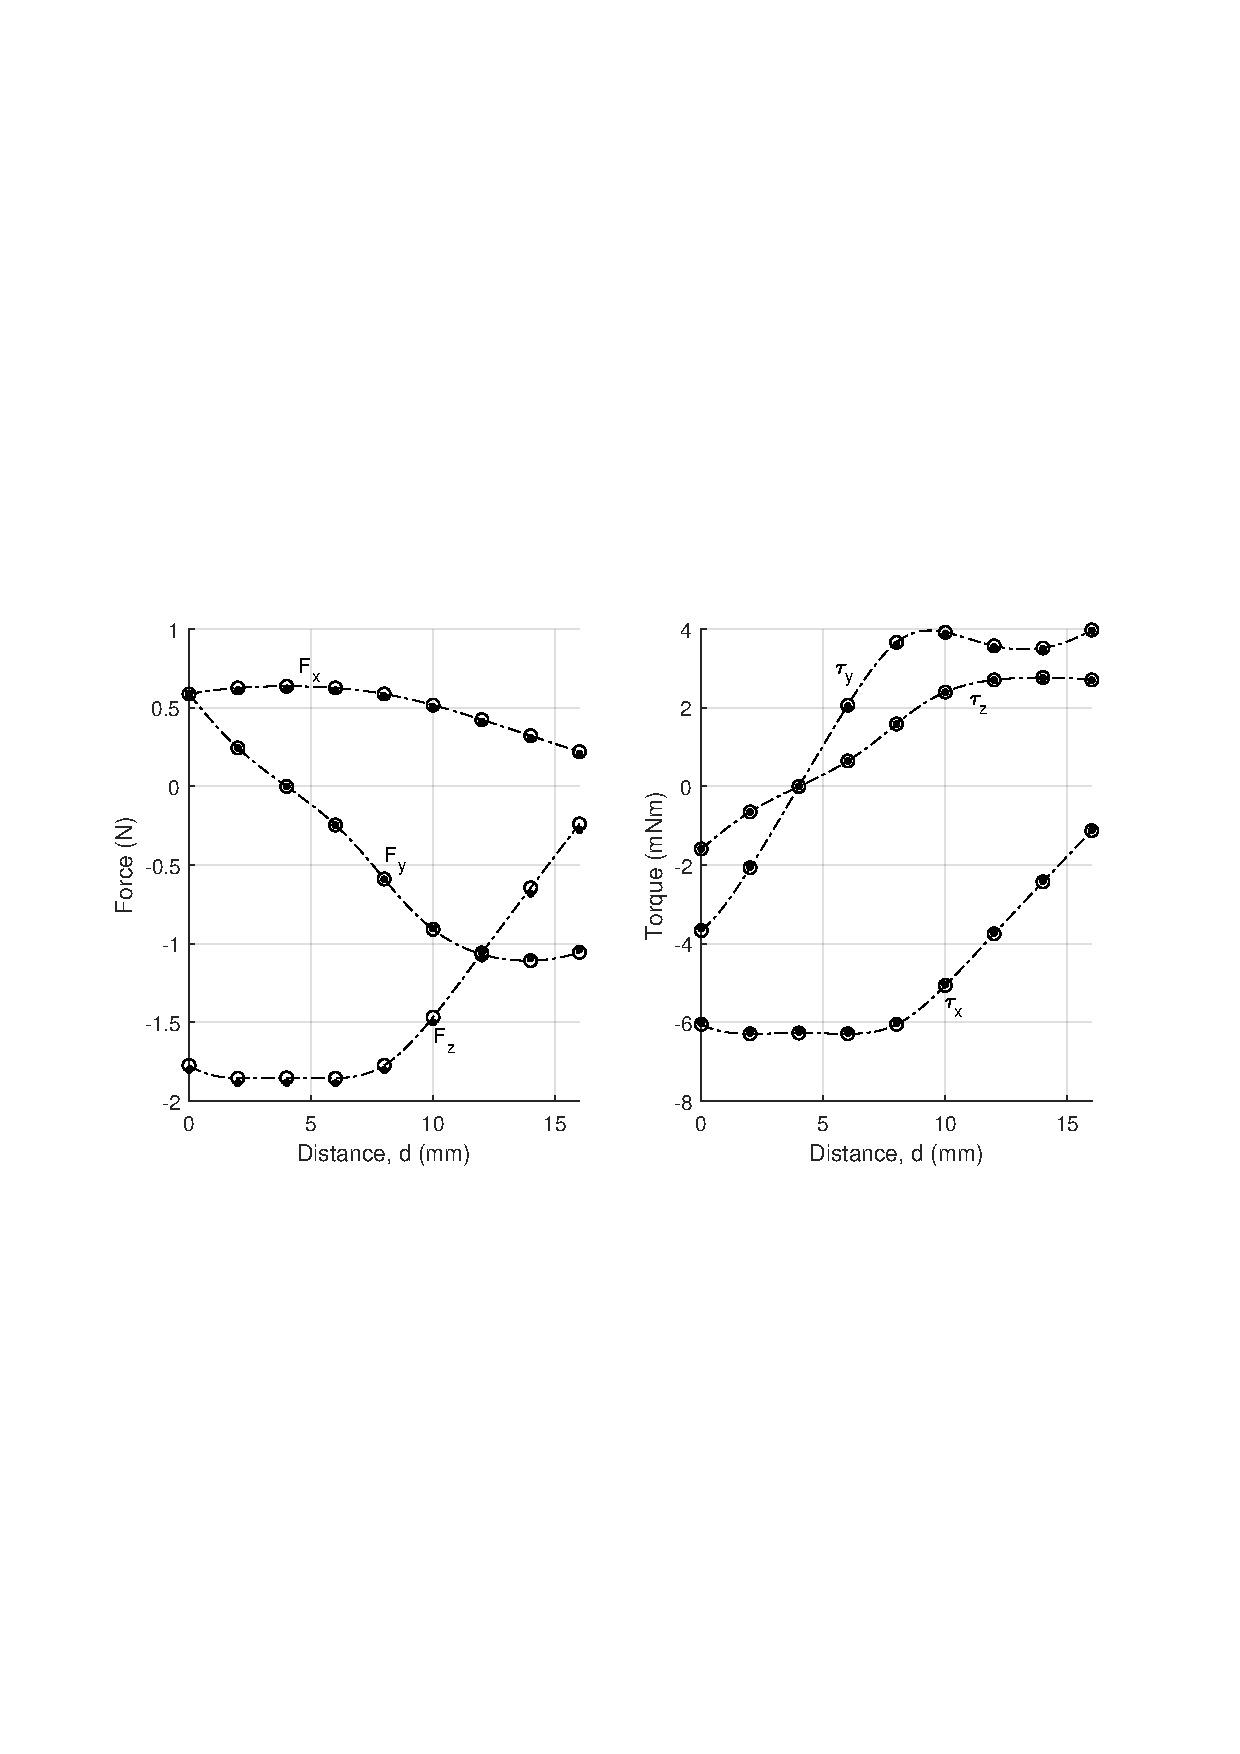
\includegraphics[trim = 3cm 9cm 3cm 9cm,width=0.9\linewidth]{p1/p1FIG4}
	\caption{Forces and torques on magnet B shown in Figure \ref{fig:p1akounyonnet} as it moves a distance \(d\) along the top of the magnet A. The dashed lines represent the results calculated from Algorithms \ref{alg:p1alg1} and \ref{alg:p1alg2}, with circles representing analytic solutions \cite{Akoun1984,Janssen2010a} and dots representing solutions obtained from a finite element simulation (Maxwell3D, ANSYS Electronics Desktop 2018.0). The values obtained with Algorithms \ref{alg:p1alg1} and \ref{alg:p1alg2} are in excellent agreement with the other two methods, especially the analytic solutions, indicating this work produces correct results for cuboidal magnets.}
	\label{fig:p1cuboidcase}
\end{figure*}

The three sets of results are shown in Figure \ref{fig:p1cuboidcase}. The forces and torques obtained from Algorithms \ref{alg:p1alg1} and \ref{alg:p1alg2} align with both the values from the finite element simulation and from the analytic solution, validating the algorithms for simple cuboidal magnets with parallel magnetisation. However, this test does not consider non-cuboidal magnets or non-parallel magnetisation and these must be considered for further validation.

Algorithms \ref{alg:p1alg1} and \ref{alg:p1alg2} were significantly faster than the finite element simulations when implemented in Matlab R2017b (MathWorks, Inc., Natick, MA, USA) on a workstation PC with an Intel Xeon E3-1240 v5 (3.50GHz) with 4 cores. Algorithms \ref{alg:p1alg1} and \ref{alg:p1alg2} completed each force calculation in approximately 0.65 seconds using 3072 triangular elements on the surface of magnet B, while the finite element simulations took a minimum of 30-40 seconds using an adaptive setup with a percent error of 1\% and approximately 17000 tetrahedral elements. Additionally, Algorithms \ref{alg:p1alg1} and \ref{alg:p1alg2} were considerably more accurate, achieving a maximum force error of 4.3 milliNewtons and a maximum torque error of 0.03 milliNewton-metres when compared to the analytic solutions, while the finite element solutions gave a maximum force error of 37 milliNewtons and a maximum torque error of 0.14 milliNewton-metres.

To validate Algorithms \ref{alg:p1alg1} and \ref{alg:p1alg2} for a more general case, two dodecahedral magnets were considered (Figure~\ref{fig:p1dodecahedra}). Both magnets are regular dodecahedra with edge lengths of 20mm and volumes of 61305mm\(^3\). Magnet B has magnetisation in the \(x\)-direction and may move vertically, while magnet A has magnetisation in the \(z\)-direction and is fixed. Both magnets have a unit magnetisation strength \(\mathbf{M}\), i.e. 1 Tesla. The \(x\)-force and \(y\)-torque on magnet B are calculated, with the torque calculated about its centre. The \(y\)- and \(z\)-forces, as well as the \(x\)- and \(z\)-torques are almost zero and thus neglected. The magnetic configuration was input into Algorithms \ref{alg:p1alg1} and \ref{alg:p1alg2} as well as a  three-dimensional finite element simulation, with the results shown in Figure \ref{fig:p1dodecahedraresults}\footnote{Due to the numeric nature of the force and torque calculations, accuracy is reduced when magnets are extremely close and an insufficient surface mesh density is used. As such, the magnets were limited to a minimum separation of 1mm.}. Due to symmetry, the forces in the \(y\) and \(z\) directions, as well as the torques about the \(x\) and \(z\) axes are extremely small and therefore not plotted in the figure.
\begin{figure*}
	\centering
	\begin{subfigure}{0.49\textwidth}
		\centering
		\tdplotsetmaincoords{70}{110}
		\begin{tikzpicture}[scale=50,tdplot_main_coords]
		\coordinate(p1t) at (0.026180,0.008506,0.005258);
		\coordinate(p2t) at (0.016181,-0.005257,-0.022270);
		\coordinate(p3t) at (0.009999,-0.013765,0.022270);
		\coordinate(p4t) at (0.000000,-0.027527,-0.005258);
		\coordinate(p5t) at (-0.000000,0.027527,0.005258);
		\coordinate(p6t) at (-0.009999,0.013765,-0.022270);
		\coordinate(p7t) at (-0.016181,0.005257,0.022270);
		\coordinate(p8t) at (-0.026180,-0.008506,-0.005258);
		\coordinate(p9t) at (0.016180,0.022271,-0.005256);
		\coordinate(p10t) at (0.010001,0.013765,-0.022270);
		\coordinate(p11t) at (-0.010001,-0.013765,0.022270);
		\coordinate(p12t) at (-0.016180,-0.022271,0.005256);
		\coordinate(p13t) at (0.016180,0.005257,0.022271);
		\coordinate(p14t) at (0.000001,-0.017012,-0.022271);
		\coordinate(p15t) at (-0.000001,0.017012,0.022271);
		\coordinate(p16t) at (-0.016180,-0.005257,-0.022271);
		\coordinate(p17t) at (0.026180,-0.008506,-0.005257);
		\coordinate(p18t) at (0.016180,-0.022271,0.005257);
		\coordinate(p19t) at (-0.016180,0.022271,-0.005257);
		\coordinate(p20t) at (-0.026180,0.008506,0.005257);
		
		\coordinate(p1b) at (0.016180,0.022270,-0.049242);
		\coordinate(p2b) at (0.016180,0.005258,-0.076770);
		\coordinate(p3b) at (0.016180,-0.005258,-0.032230);
		\coordinate(p4b) at (0.016180,-0.022270,-0.059758);
		\coordinate(p5b) at (-0.016180,0.022270,-0.049242);
		\coordinate(p6b) at (-0.016180,0.005258,-0.076770);
		\coordinate(p7b) at (-0.016180,-0.005258,-0.032230);
		\coordinate(p8b) at (-0.016180,-0.022270,-0.059758);
		\coordinate(p9b) at (0.000000,0.027528,-0.059756);
		\coordinate(p10b) at (0.000000,0.017014,-0.076770);
		\coordinate(p11b) at (0.000000,-0.017014,-0.032230);
		\coordinate(p12b) at (0.000000,-0.027528,-0.049244);
		\coordinate(p13b) at (0.010000,0.013763,-0.032229);
		\coordinate(p14b) at (0.010000,-0.013763,-0.076771);
		\coordinate(p15b) at (-0.010000,0.013763,-0.032229);
		\coordinate(p16b) at (-0.010000,-0.013763,-0.076771);
		\coordinate(p17b) at (0.026180,0.008507,-0.059757);
		\coordinate(p18b) at (0.026180,-0.008507,-0.049243);
		\coordinate(p19b) at (-0.026180,0.008507,-0.059757);
		\coordinate(p20b) at (-0.026180,-0.008507,-0.049243);
		
		\draw[fill=white] (p3b) -- (p11b) -- (p7b) -- (p15b) -- (p13b) -- cycle;
		\draw[fill=white] (p11b) -- (p12b) -- (p4b) -- (p18b) -- (p3b) -- cycle;
		\draw[fill=white] (p3b) -- (p13b) -- (p1b) -- (p17b) -- (p18b) -- cycle;
		\draw[fill=white] (p13b) -- (p15b) -- (p5b) -- (p9b) -- (p1b) -- cycle;
		\draw[fill=white] (p18b) -- (p17b) -- (p2b) -- (p14b) -- (p4b) -- cycle;
		\draw[fill=white] (p1b) -- (p17b) -- (p2b) -- (p10b) -- (p9b) -- cycle;
		
		\draw[fill=white] (p11t) -- (p3t) -- (p13t) -- (p15t) -- (p7t) -- cycle;
		\draw[fill=white] (p3t) -- (p18t) -- (p17t) -- (p1t) -- (p13t) -- cycle;
		\draw[fill=white] (p1t) -- (p9t) -- (p5t) -- (p15t) -- (p13t) -- cycle;
		\draw[fill=white] (p1t) -- (p9t) -- (p10t) -- (p2t) -- (p17t) -- cycle;
		\draw[fill=white] (p18t) -- (p17t) -- (p2t) -- (p14t) -- (p4t) -- cycle;
		\draw[fill=white] (p9t) -- (p5t) -- (p19t) -- (p6t) -- (p10t) -- cycle;
		
		
		\node(A) at (0,0,-0.0525) {\text{A}};
		\node(B) at (0,0.012,0.005) {\text{B}};
		\end{tikzpicture}
		\caption{}
	\end{subfigure}
	~%\hspace{20pt}
	\begin{subfigure}{0.49\textwidth}
		\centering
		\tdplotsetmaincoords{90}{180}
		\begin{tikzpicture}[scale=50,tdplot_main_coords]
		\coordinate(p1t) at (0.026180,0.008506,0.005258);
		\coordinate(p2t) at (0.016181,-0.005257,-0.022270);
		\coordinate(p3t) at (0.009999,-0.013765,0.022270);
		\coordinate(p4t) at (0.000000,-0.027527,-0.005258);
		\coordinate(p5t) at (-0.000000,0.027527,0.005258);
		\coordinate(p6t) at (-0.009999,0.013765,-0.022270);
		\coordinate(p7t) at (-0.016181,0.005257,0.022270);
		\coordinate(p8t) at (-0.026180,-0.008506,-0.005258);
		\coordinate(p9t) at (0.016180,0.022271,-0.005256);
		\coordinate(p10t) at (0.010001,0.013765,-0.022270);
		\coordinate(p11t) at (-0.010001,-0.013765,0.022270);
		\coordinate(p12t) at (-0.016180,-0.022271,0.005256);
		\coordinate(p13t) at (0.016180,0.005257,0.022271);
		\coordinate(p14t) at (0.000001,-0.017012,-0.022271);
		\coordinate(p15t) at (-0.000001,0.017012,0.022271);
		\coordinate(p16t) at (-0.016180,-0.005257,-0.022271);
		\coordinate(p17t) at (0.026180,-0.008506,-0.005257);
		\coordinate(p18t) at (0.016180,-0.022271,0.005257);
		\coordinate(p19t) at (-0.016180,0.022271,-0.005257);
		\coordinate(p20t) at (-0.026180,0.008506,0.005257);
		
		\coordinate(p1b) at (0.016180,0.022270,-0.049242);
		\coordinate(p2b) at (0.016180,0.005258,-0.076770);
		\coordinate(p3b) at (0.016180,-0.005258,-0.032230);
		\coordinate(p4b) at (0.016180,-0.022270,-0.059758);
		\coordinate(p5b) at (-0.016180,0.022270,-0.049242);
		\coordinate(p6b) at (-0.016180,0.005258,-0.076770);
		\coordinate(p7b) at (-0.016180,-0.005258,-0.032230);
		\coordinate(p8b) at (-0.016180,-0.022270,-0.059758);
		\coordinate(p9b) at (0.000000,0.027528,-0.059756);
		\coordinate(p10b) at (0.000000,0.017014,-0.076770);
		\coordinate(p11b) at (0.000000,-0.017014,-0.032230);
		\coordinate(p12b) at (0.000000,-0.027528,-0.049244);
		\coordinate(p13b) at (0.010000,0.013763,-0.032229);
		\coordinate(p14b) at (0.010000,-0.013763,-0.076771);
		\coordinate(p15b) at (-0.010000,0.013763,-0.032229);
		\coordinate(p16b) at (-0.010000,-0.013763,-0.076771);
		\coordinate(p17b) at (0.026180,0.008507,-0.059757);
		\coordinate(p18b) at (0.026180,-0.008507,-0.049243);
		\coordinate(p19b) at (-0.026180,0.008507,-0.059757);
		\coordinate(p20b) at (-0.026180,-0.008507,-0.049243);
		
		\draw[gray,fill=white] (p7t) -- (p11t) -- (p12t) -- (p8t) -- (p20t) -- cycle;
		\draw[gray,fill=white] (p11t) -- (p3t) -- (p18t) -- (p4t) -- (p12t) -- cycle;
		\draw[gray,fill=white] (p3t) -- (p13t) -- (p1t) -- (p17t) -- (p18t) -- cycle;
		\draw[gray,fill=white] (p18t) -- (p17t) -- (p2t) -- (p14t) -- (p4t) -- cycle;
		\draw[gray,fill=white] (p12t) -- (p4t) -- (p14t) -- (p16t) -- (p8t) -- cycle;
		
		\draw[gray,fill=white] (p7b) -- (p11b) -- (p12b) -- (p8b) -- (p20b) -- cycle;
		\draw[gray,fill=white] (p11b) -- (p3b) -- (p18b) -- (p4b) -- (p12b) -- cycle;
		\draw[gray,fill=white] (p12b) -- (p4b) -- (p14b) -- (p16b) -- (p8b) -- cycle;
		\draw[gray,fill=white] (p20b) -- (p8b) -- (p16b) -- (p6b) -- (p19b) -- cycle;
		\draw[gray,fill=white] (p18b) -- (p17b) -- (p2b) -- (p14b) -- (p4b) -- cycle;
		
		\draw[->,thick] (-0.01,0,0) -- (0.01,0,0);
		\draw[->,thick] (0,0,-0.0645) -- (0,0,-0.0445);
		
		\draw[<->,black] (-0.025,0,-0.0223) -- (-0.025,0,-0.0322);
		
		\node(M2) at (0,0,0.004){\(\mathbf{M}\)};
		\node(M1) at (-0.005,0,-0.0545){\(\mathbf{M}\)};
		\node(d) at (-0.03,0,-0.0272){\(d\)};
		\node(A) at (-0.03,0,-0.0545) {\text{A}};
		\node(B) at (-0.03,0,0) {\text{B}};
		
		\draw[->] (-0.065,0,0) -- (-0.05,0,0);
		\draw[->] (-0.065,0,0) -- (-0.065,0,0.015);
		\node(x) at (-0.045,0,0) {\(x\)};
		\node(z) at (-0.065,0,0.02) {\(z\)};
		\end{tikzpicture}
		\caption{}
	\end{subfigure}
	\caption{Three-dimensional view (a) and side view (b) of two dodecahedral permanent magnets, with magnet B positioned vertically above magnet A. They have perpendicular magnetisation, with magnet A having vertical magnetisation and magnet B having horizontal magnetisation. Magnet B moves a distance \(d\) in the vertical direction, with the forces and torques being calculated as it moves.}
	\label{fig:p1dodecahedra}
\end{figure*}
\begin{figure*}
	\centering
	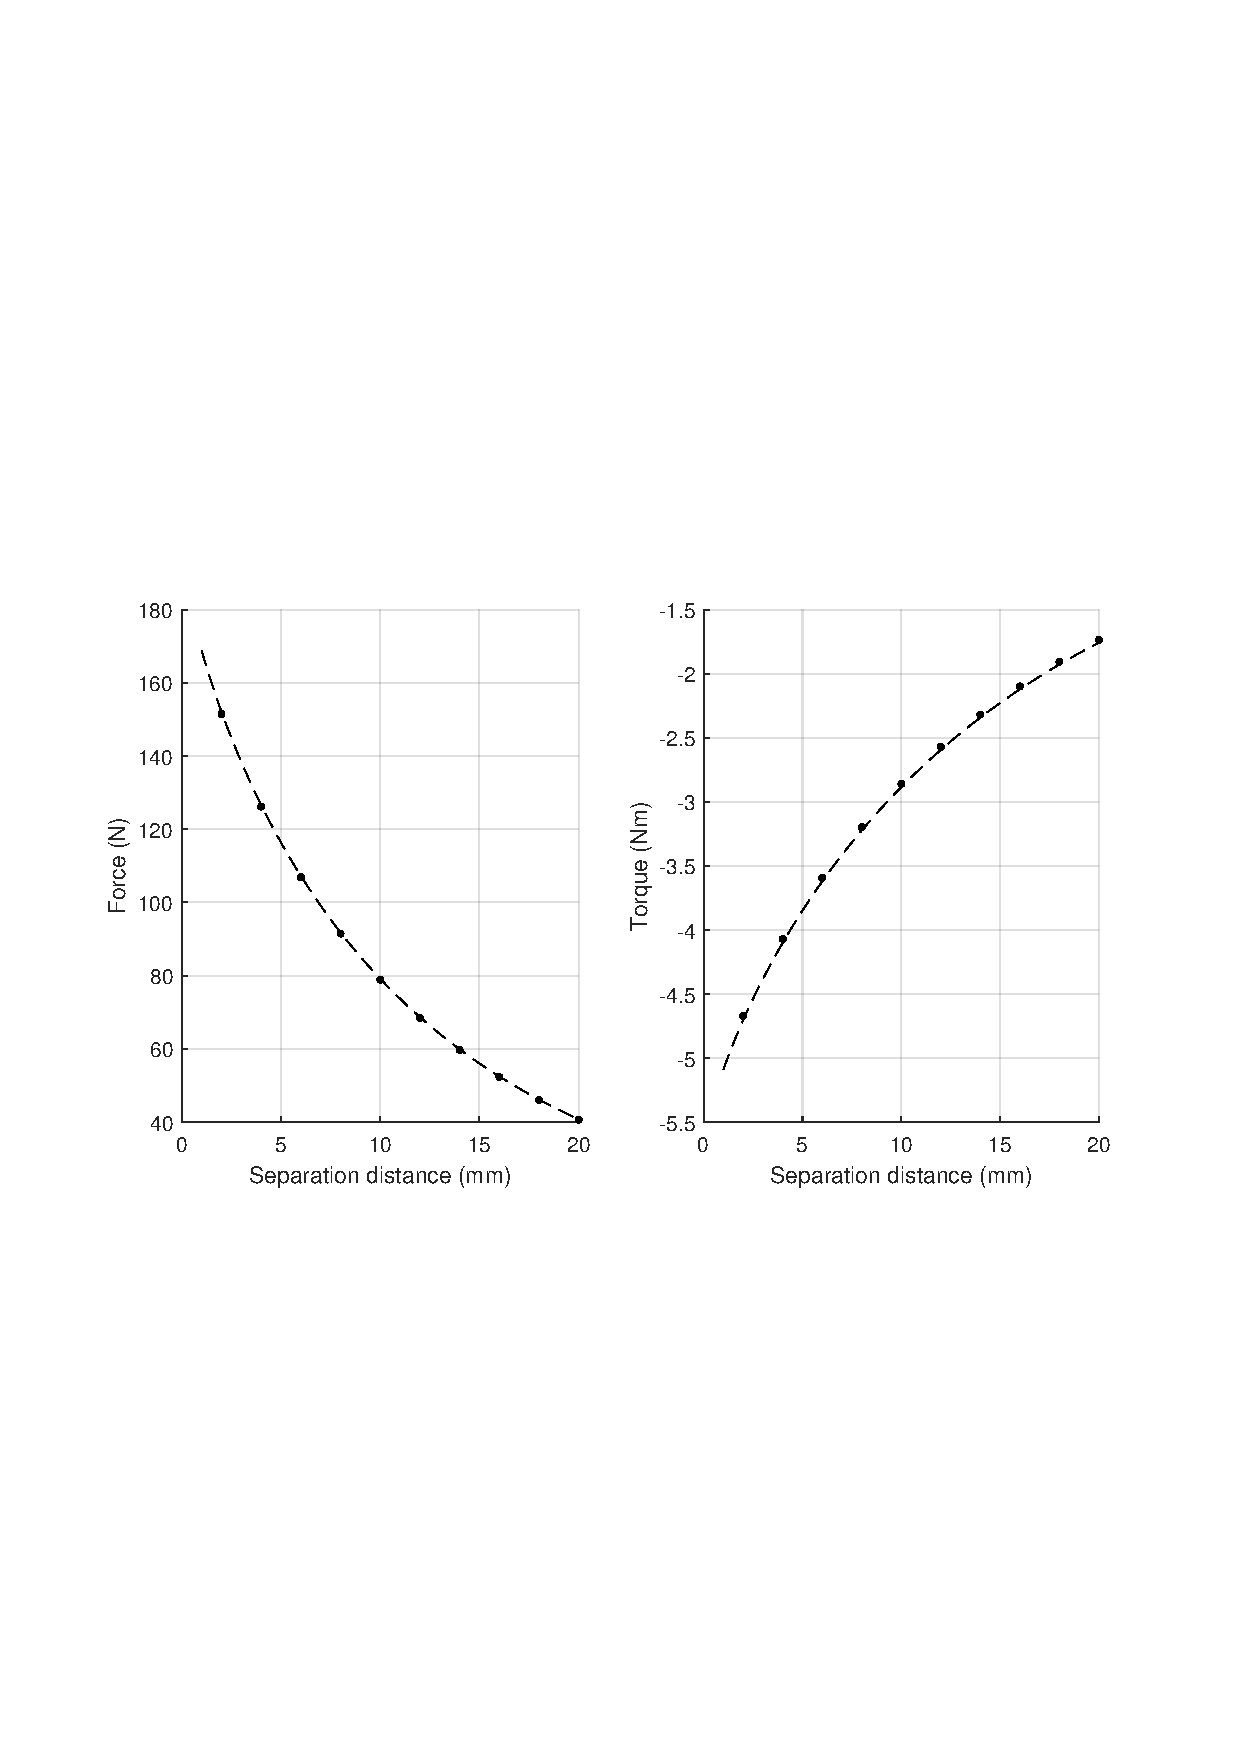
\includegraphics[trim = 3cm 9cm 3cm 9cm,width=0.9\linewidth]{p1/p1FIG6}
	\caption{The \(x\)-force and \(y\)-torque on magnet B shown in Figure \ref{fig:p1dodecahedra}. Both magnets are regular dodecahedra with edge lengths of 20mm. The torque is evaluated about the centre of magnet B. Dashed lines represent the force and torque evaluated using Algorithms \ref{alg:p1alg1} and \ref{alg:p1alg2}, and dots represent the results from finite element simulations. The results from both methods are in agreement, indicating correct results from Algorithms \ref{alg:p1alg1} and \ref{alg:p1alg2}.}
	\label{fig:p1dodecahedraresults}
\end{figure*}

The results obtained from Algorithms \ref{alg:p1alg1} and \ref{alg:p1alg2} align well with the finite element simulations. This indicates that the algorithms produce accurate force and torque results for non-cuboidal polyhedral magnets with non-parallel magnetisation vectors, further validating Algorithms \ref{alg:p1alg1} and \ref{alg:p1alg2}.

No analytic solutions for dodecahedral permanent magnets exist, so the error of Algorithms \ref{alg:p1alg1}, \ref{alg:p1alg2}, and the finite element simulations cannot be quantified. However, the solution time can still be analysed. Algorithms \ref{alg:p1alg1} and \ref{alg:p1alg2} were again considerably faster than the finite element simulations, with solutions being completed in approximately 4.96 seconds using 4608 triangular elements on the surface of magnet B, while each finite element simulation took approximately 40-50 seconds using an adaptive setup with a percent error of 1\% and approximately 18000 tetrahedral elements.
\section{Geometric optimisation}\label{sec:p1geometricOptimisation}
Algorithms \ref{alg:p1alg1} and \ref{alg:p1alg2} can be used for fast optimisation of magnetic systems. Presented here is one such case, wherein two pyramidal frustums are arranged with magnet B above magnet A, as shown in Figure \ref{fig:p1frustumcase}. Both magnets have a unit magnetisation strength of 1 Tesla. The magnetisation vectors are oppositely directed with the magnets in repulsion. The wall angle \(\theta\) is varied to maximise the force at a given distance while the magnet height and volume are kept constant at 5cm and 500cm\(^3\) respectively. A wall angle of \(\theta = 90^\circ\) corresponds to a cuboidal magnet with a height of 5cm and both width and depth of 10cm.
\begin{figure*}
	\centering
	\begin{subfigure}{0.4\textwidth}
		\centering
		\tdplotsetmaincoords{70}{110}
		\begin{tikzpicture}[scale=40,tdplot_main_coords]
		\coordinate(p1t) at (-0.050000,-0.050000,-0.000000);
		\coordinate(p2t) at (-0.050000,0.050000,-0.000000);
		\coordinate(p3t) at (0.050000,-0.050000,-0.000000);
		\coordinate(p4t) at (0.050000,0.050000,-0.000000);
		\coordinate(p5t) at (-0.025000,-0.025000,0.050000);
		\coordinate(p6t) at (0.025000,-0.025000,0.050000);
		\coordinate(p7t) at (-0.025000,0.025000,0.050000);
		\coordinate(p8t) at (0.025000,0.025000,0.050000);
		
		\coordinate(p1b) at (0.050000,0.050000,-0.025000);
		\coordinate(p2b) at (0.050000,-0.050000,-0.025000);
		\coordinate(p3b) at (-0.050000,0.050000,-0.025000);
		\coordinate(p4b) at (-0.050000,-0.050000,-0.025000);
		\coordinate(p5b) at (0.025000,0.025000,-0.075000);
		\coordinate(p6b) at (-0.025000,0.025000,-0.075000);
		\coordinate(p7b) at (0.025000,-0.025000,-0.075000);
		\coordinate(p8b) at (-0.025000,-0.025000,-0.075000);
		
		\draw[fill=white] (p4b) -- (p3b) -- (p1b) -- (p2b) -- cycle;
		\draw[fill=white] (p1b) -- (p3b) -- (p6b) -- (p5b) -- cycle;
		\draw[fill=white] (p1b) -- (p2b) -- (p7b) -- (p5b) -- cycle;
		
		\draw[fill=white] (p5t) -- (p6t) -- (p8t) -- (p7t) -- cycle;
		\draw[fill=white] (p2t) -- (p4t) -- (p8t) -- (p7t) -- cycle;
		\draw[fill=white] (p6t) -- (p8t) -- (p4t) -- (p3t) -- cycle;
		
		\node(A) at (-0.0375,-0.025,-0.08) {\text{A}};
		\node(B) at (-0.0375,-0.025,-0.005) {\text{B}};
		\end{tikzpicture}
		\caption{}
	\end{subfigure}
	~ \hspace{20pt}
	\begin{subfigure}{0.4\textwidth}
		\centering
		\tdplotsetmaincoords{90}{0}
		\begin{tikzpicture}[scale=40,tdplot_main_coords]
		\coordinate(p1t) at (-0.050000,-0.050000,-0.000000);
		\coordinate(p2t) at (-0.050000,0.050000,-0.000000);
		\coordinate(p3t) at (0.050000,-0.050000,-0.000000);
		\coordinate(p4t) at (0.050000,0.050000,-0.000000);
		\coordinate(p5t) at (-0.025000,-0.025000,0.050000);
		\coordinate(p6t) at (0.025000,-0.025000,0.050000);
		\coordinate(p7t) at (-0.025000,0.025000,0.050000);
		\coordinate(p8t) at (0.025000,0.025000,0.050000);
		
		\coordinate(p1b) at (0.050000,0.050000,-0.025000);
		\coordinate(p2b) at (0.050000,-0.050000,-0.025000);
		\coordinate(p3b) at (-0.050000,0.050000,-0.025000);
		\coordinate(p4b) at (-0.050000,-0.050000,-0.025000);
		\coordinate(p5b) at (0.025000,0.025000,-0.075000);
		\coordinate(p6b) at (-0.025000,0.025000,-0.075000);
		\coordinate(p7b) at (0.025000,-0.025000,-0.075000);
		\coordinate(p8b) at (-0.025000,-0.025000,-0.075000);
		
		\draw[gray] (p2b) -- (p4b) -- (p8b) -- (p7b) -- cycle;
		\draw[gray] (p1t) -- (p3t) -- (p6t) -- (p5t) -- cycle;
		
		\draw[<->] (0,0,-0.025) -- (0,0,0);
		\node (d) at (0.005,0,-0.0125) {\(d\)};
		
		\draw[->,thick] (0,0,0.035) -- (0,0,0.015);
		\node (M1) at (-0.0075,0,0.025) {\textbf{M}};
		\draw[->,thick] (0,0,-0.06) -- (0,0,-0.04);
		\node (M2) at (-0.0075,0,-0.05) {\textbf{M}};
		
		\node(theta1) at (-0.022,0,0.043){\(\theta\)};
		\node(theta2) at (-0.022,0,-0.068){\(\theta\)};
		\node(A) at (0.025,0,-0.05) {\text{A}};
		\node(B) at (0.025,0,0.025) {\text{B}};
		
		\end{tikzpicture}
		\caption{}
	\end{subfigure}
	\caption{Three-dimensional view (a) and side view (b) of two pyramidal frustum magnets with opposing vertical magnetisations \(\mathbf{M}\). Magnet B moves a distance \(d\) in the vertical direction. The wall angle \(\theta\) is varied while maintaining a constant magnet volume and height.}
	\label{fig:p1frustumcase}
\end{figure*}

The frustums were separated by a given distance \(d\) and the wall angle \(\theta\) varied. For all values of \(\theta\), the repulsive force between the magnets was calculated and divided by the maximum force for each separation to give the normalised force plot shown in Figure \ref{fig:p1frustumforce}. The peaks of this plot correspond to the maximum force at a given separation distance, and hence show the optimal wall angle for that distance. The optimal angle was calculated for several separation distances using this method with the results shown in Table \ref{tab:p1optimalfrustum}. It can be seen that the optimal wall angle increases with separation distance, indicating that as the magnets move further apart, the optimal shape tends toward a pyramid. On the contrary, as the magnets become closer, the optimal shape tends toward a cuboid.
\begin{figure}
	\centering
	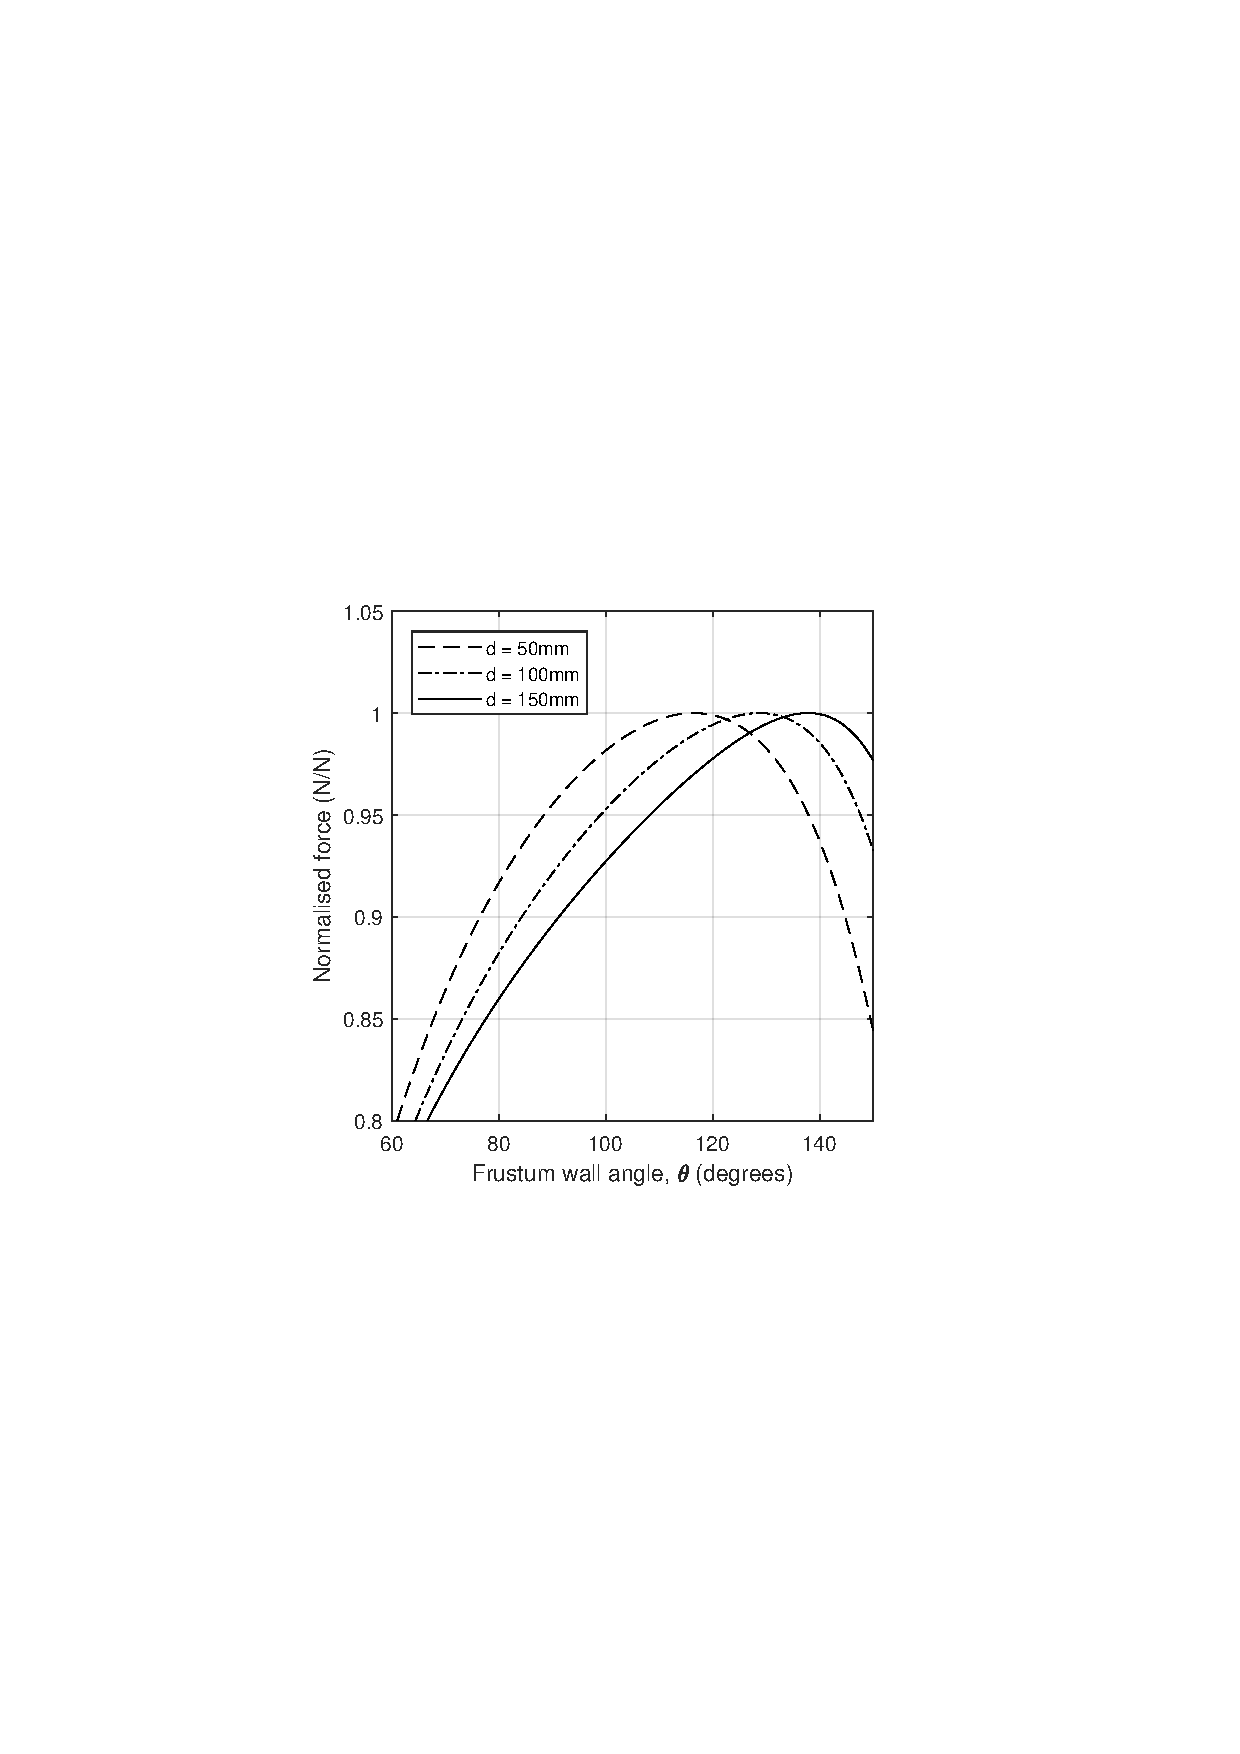
\includegraphics[trim = 5cm 9cm 5cm 9cm,width=0.8\linewidth]{p1/p1FIG8}
	\caption{The normalised force between the two frustum magnets shown in Figure \ref{fig:p1frustumcase} as the wall angle \(\theta\) is varied. Each plot corresponds to a given separation distance \(d\) shown in the legend. The normalised force is calculated by dividing the force at each point by the maximum force for each separation distance. The peak of each plot corresponds to the maximum force attained, and thus the optimal wall angle. As the separation distance increases, the peak moves to the right, indicating the optimum wall angle increases with the separation distance.}
	\label{fig:p1frustumforce}
\end{figure}
\begin{table}
	\centering
	\caption{The optimal wall angle of the pyramidal frustums at a given distance. This angle maximises the repulsive force between the magnets while maintaining a constant magnet volume and height.}
	\begin{tabular}{cc}
		\hline
		Separation distance (mm) & Optimal angle (degrees) \\
		\hline
		25 & 110 \\
		50 & 117 \\
		75 & 123 \\
		100 & 129 \\
		125 & 134 \\
		150 & 138 \\
		\hline
		\label{tab:p1optimalfrustum}
	\end{tabular}
\end{table}

The above test lead to an investigation on optimal angle for a varying separation distance. For a given separation distance, a golden ratio search was implemented to find the optimal angle which maximises the repulsive force. This was repeated for a large range of separation distances, and the plot shown in Figure \ref{fig:p1optimalfrustum} (left) was obtained. Again, it can be seen that the optimal angle increases with the separation distance. Interestingly, when the separation distance is zero, the optimal angle is not 90\(^\circ\). Namely, the optimal geometry is not cuboidal when the magnets are touching. Furthermore, the optimal angle is always greater than 90\(^\circ\), implying that cuboidal magnets are not the optimal geometry for this particular configuration.
\begin{figure*}
	\centering
	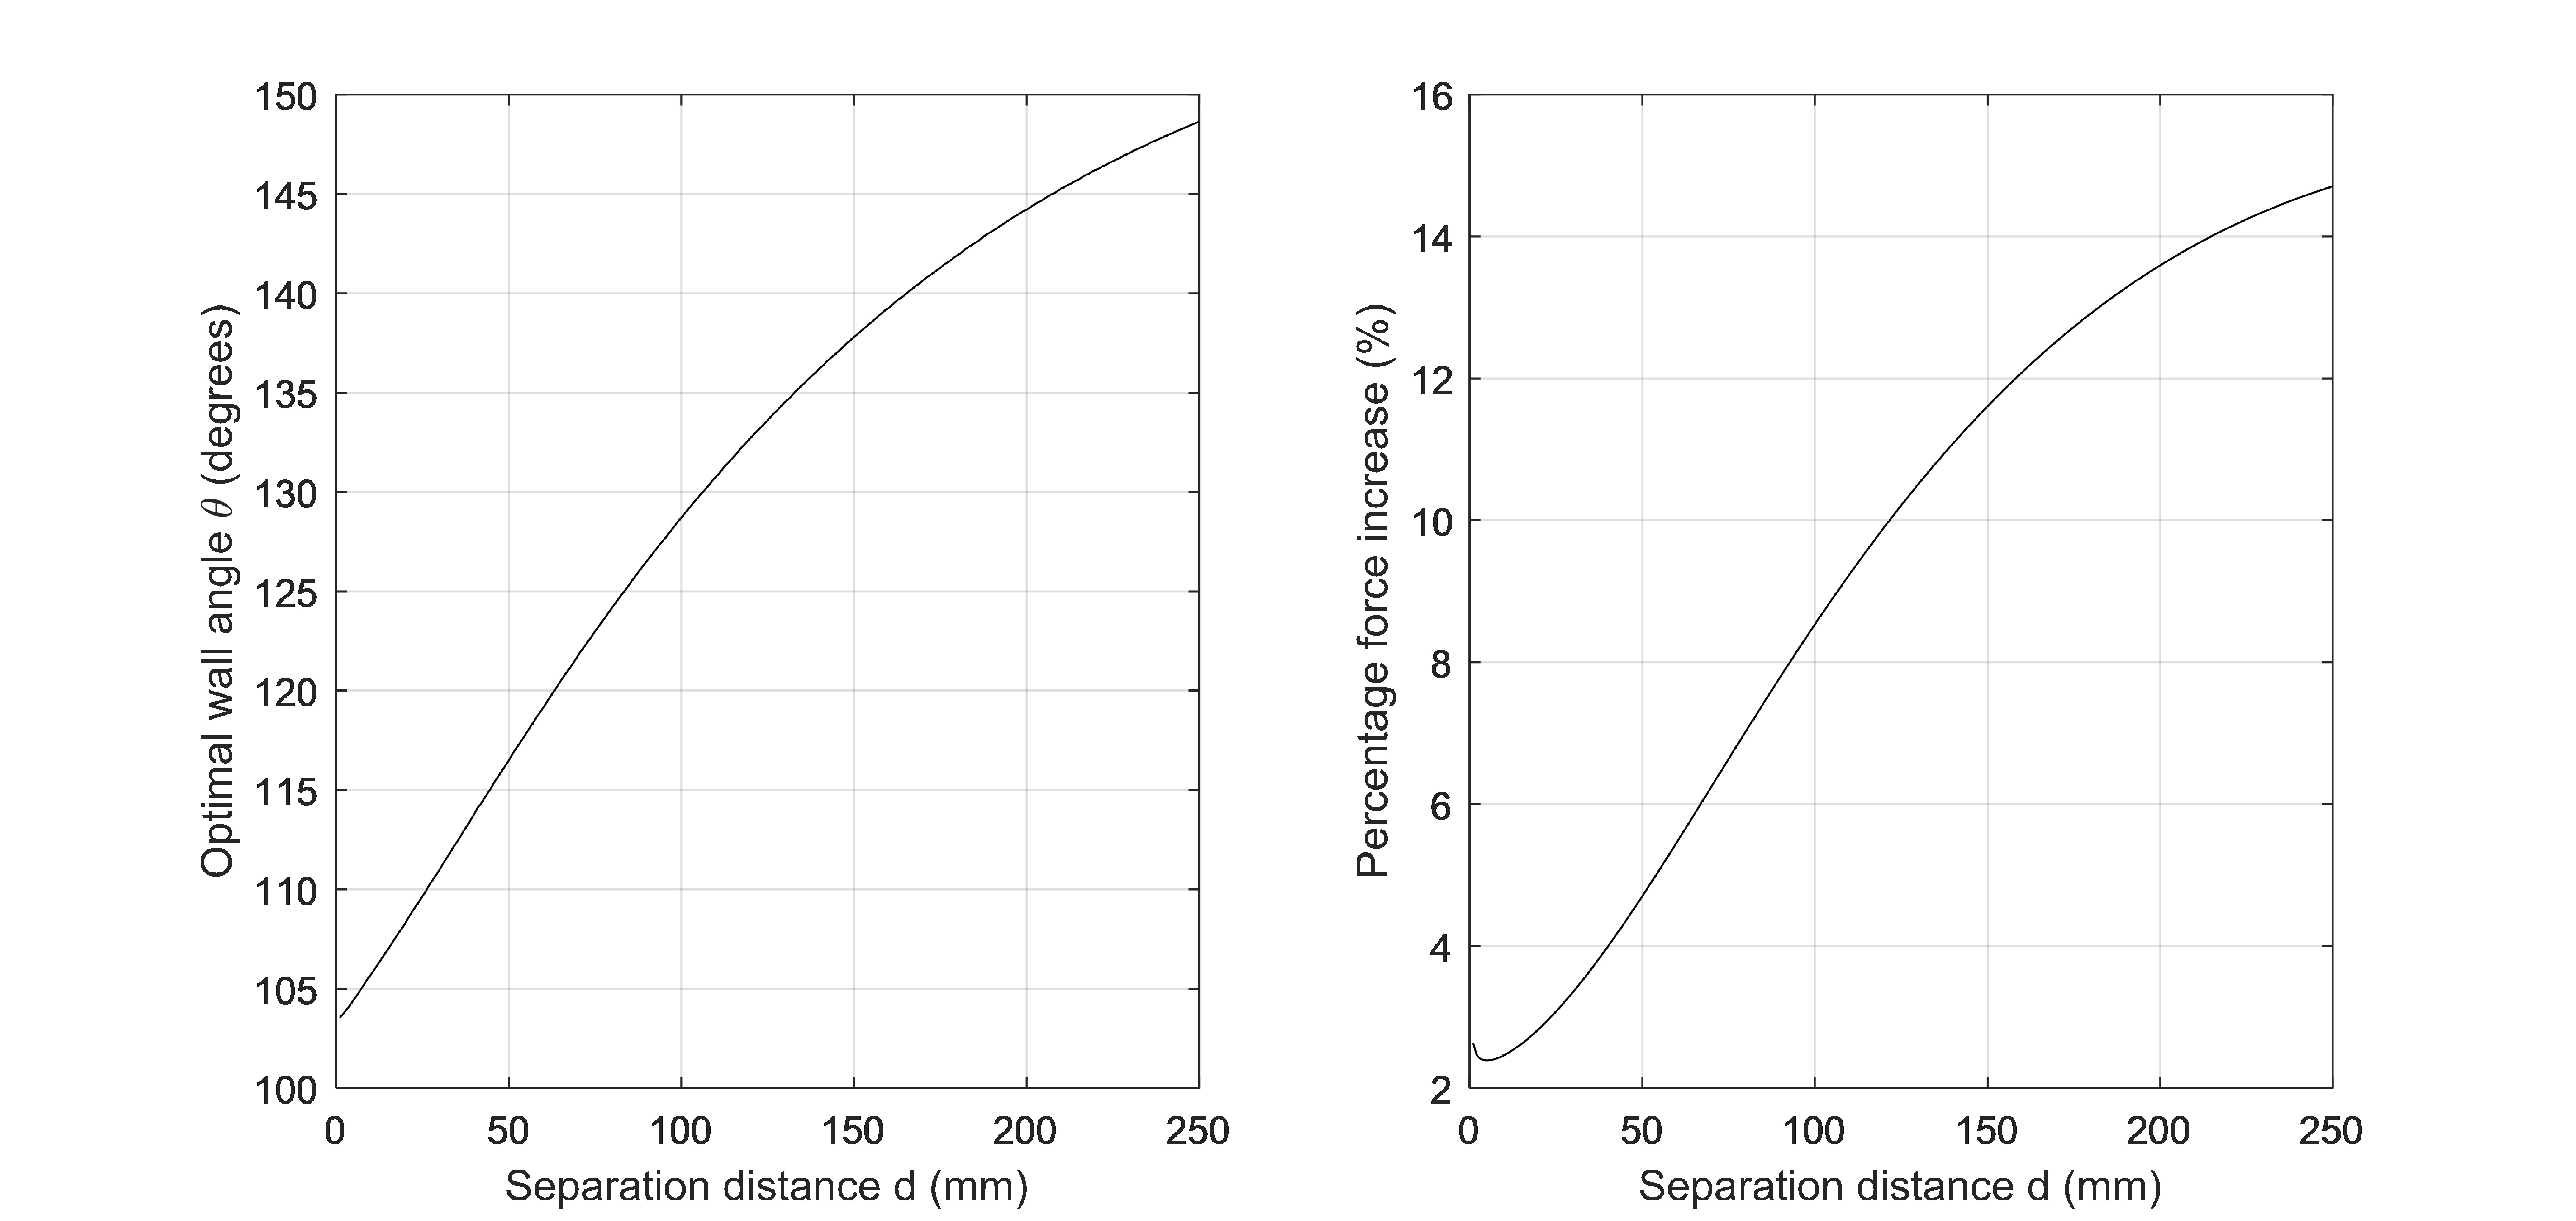
\includegraphics[trim = 4cm 0cm 4cm 0cm,width=\linewidth]{p1/p1FIG9}
	\caption{The optimal wall angle \(\theta\) of the frustums at a given distance to maximise the repulsive force between them (left). At all separation distances, the optimal angle is larger than 90\(^\circ\), indicating a cuboid is never the optimal geometry in this case. The optimal angle increases with separation distance, and tends toward a pyramid geometry at large separations. These results were compared to two cuboidal magnets with equal volume and height at the same separation distances. The force increase as a percentage of the repulsive force between the cuboids was found (right). A considerable increase in force was found, especially at larger separations. This implies that a larger force can be achieved with smaller mass if the system is optimised.}
	\label{fig:p1optimalfrustum}
\end{figure*}

In addition to calculating the optimal angle at a given separation distance, the percentage force increase was calculated. For each separation distance, the maximum force was found, as well as the force between two cuboidal magnets of equivalent height and volume. The percentage force increase is defined as
\begin{equation}
\text{PFI} = \frac{F_\text{frustum}-F_\text{cuboid}}{F_\text{cuboid}} \times 100\% \text{.}
\end{equation}
This percentage force increase was plotted against separation distance (Figure \ref{fig:p1optimalfrustum}, right). This value increases with separation distance, corresponding to a larger wall angle. Additionally, the force increase is positive for all separation distances, meaning with a constant magnetic volume, polyhedral magnets can achieve larger forces than cuboidal magnets. Alternatively, the same forces can be achieved using a smaller system mass, which could lead to significant cost savings.
\section{Conclusion}\label{sec:p1conclusion}
Permanent magnets are widely used in many industries and as such it is useful to characterise the interactions between them. This paper has outlined a fast semi-analytic method to calculate magnetic fields, forces, and torques of polyhedral permanent magnets. The development of two algorithms were discussed and implemented in Matlab. Several validation cases were considered, including a basic cuboid case and a more complicated system with dodecahedral magnets. These results were then validated against both literature (where possible) and finite element simulations. Then, a system with two pyramidal frustums was implemented in which the wall angle and separation distance could be varied while maintaining constant magnetic volume and height. The algorithms presented in this paper were used for rapid optimisation\footnote{Here, optimisation refers to maximising the force between two magnets of constant volume by varying magnet geometry. However, many forms of optimisation, such as optimisation of force per unit magnet height or torque per unit mass, may be used.} of this system, maximising the force between the magnets at a given distance. This resulted in the optimal angle being calculated over a large number of separations. Additionally, a considerable improvement in force over cuboidal magnets was found, showing standard magnetic geometries are not always optimal. The algorithms presented here can be used to further understand non-standard magnetic geometries, as well as optimise magnetic systems quickly to increase their performance.
\clearpage
\section*{Author's remarks on Chapter \ref{chap:paper1}}
The field equations presented in this chapter enable the evaluation of the magnetic field due to any polyhedral permanent magnet with constant uniform magnetisation and a relative permeability of unity. However, the methodology has several limitations that reduce the effectiveness of field evaluation. The most significant limitation is that of scaling; if the number of points at which the field is calculated is doubled, the methodology will take approximately twice as long to evaluate the field. This is because the entire process, including the deconstruction of the geometry, must be performed uniquely for each field point. In many situations, a large number of field points is desired, such as estimating forces and torques, optimising the field due to a magnet array (Chapter \ref{chap:paper3}), or modelling magnetic permeability (Chapter \ref{chap:paper4}). In addition, singularities in the equations exist for points on the same plane as the magnet facets. These limitations necessitate an alternative methodology which scales well with many field calculations and includes treatment of any singularities in the field equations.

\newpage
\section*{References}
\addcontentsline{toc}{section}{\protect\numberline{}References}
\printbibliography[heading=none]